% PREAMBLE
\documentclass[12pt, letterpaper]{article}
\usepackage[utf8]{inputenc}
\usepackage{tipa}
\usepackage[margin=1in]{geometry}
\usepackage[parfill]{parskip}
\usepackage{hyperref}
\usepackage{graphicx}
\title{Pronunciation Checking with ASR\\ \small Detailed Specification}
\author{Evan Nichols}
\date{MFF 2021/2022}

\begin{document}
\maketitle

\section*{Main Idea}
The goal of this project is to present the user with a simple application that will allow them to submit recorded speech and receive a score based on their pronunciation. The application will be built using Flask, a web application framework in Python. The main computational part of the app will be using NVIDIA's NeMo toolkit, which provides the neural network module that actually grades the speech input. The application consists of a web page run in JavaScript, and a back end in Python, which uses the NN to process speech. 

\section*{Interface}
When looking at the webpage the user will see several elements:
\begin{itemize}
\item A drop-down list selection of XML library files that hold the speech prompt phrases.

\item A numbered selection which pulls a phrase from the selected XML library.

\item \textbf{Record} begins recording audio. The user should read the selected phrase (displayed in the text box above) aloud and press \textbf{Stop} when finished. The audio player to the right allows the user to preview their recorded audio, and the user is able to overwrite the current input by simply recording again. Upon recording, the app also creates a text file which contains the prompt. Once the recording stops, the app prepares the data set which will be used by the ASR module. This involves reformatting the audio via \textit{ffmpeg}, and storing the audio file name, the audio's duration, and the selected phrase in a JSON file, which consists of one line that matches the following format: \\
\hspace*{19mm} \{"audio\_filename": \textit{"file.wav"}, "duration": \textit{1.00}, "text": \textit{"Text."}\} \\
This file is read by the neural network module, which creates another file with a percentage score and text keys. Also, a spectrogram of the recorded audio is displayed at the bottom of the page.

\item \textbf{Grade} parses the resulting text file created by the ASR module and displays it to the user. It uses Phonemizer to show the user both regular text and the phonetic representation of their speech.
\end{itemize}
\newpage%######################################################################


\section*{Tools \& Dependencies}
The application uses the latest version of Python3.\\
Packages and tools were installed using the \textbf{Pip} package manager for Python (version 20.3.1 at the time of writing). Some installations may fail if an older version is used.

\textbf{Flask} is an extensible "micro" web framework in Python. Here Flask is used to enable request dispatching between the front and back ends. It may be necessary to also use Flask-CORS (Cross Origin Resource Sharing) to bypass the security stops of some browsers. Chromium-based browsers, for example, will likely require this inclusion.
\\To install: \textit{pip install Flask}
\\\hspace*{19mm} \textit{pip install -U flask-cors}
%https://flask.palletsprojects.com/en/1.1.x/
%https://github.com/corydolphin/flask-cors

\textbf{NeMo} is a toolkit for applications of Conversational AI. It includes extendable collections of pre-made modules and pre-trained models for automatic speech recognition, natural language processing, and text-to-speech. NeMo can utilize NVIDIA's Tensor Cores and is able to be scaled out to multiple GPUs. The current version of NeMo requires Pytorch 1.7.1, which defines the Tensor class that allows storing and operating on multidimensional rectangular arraysof numbers on CUDA-capable NVIDIA GPUs.
\\To install: \textit{pip install Cython}
\\\hspace*{19mm} \textit{pip install nemo-toolkit==1.0.0b3}
\\\hspace*{19mm} \textit{pip install torch torchvision torchaudio}

\textbf{ffmpeg} is a command-line tool used to convert multimedia files between formats. In this application, the command used is \textit{ffmpeg -i input\_file.* -ar 16000 -ac 1 output.wav}. Here, \textit{-ar 16000} specifies the sampling frequency (which is the same as the input stream by default) and \textit{-ac 1} specifies the number of audio channels. Reformatting the audio input with this command prepares it for processing by the neural network module. This command is always run, even when it may be redundant.
\\To install: \textit{pip install python-ffmpeg}
%https://ffmpeg.org/

\textbf{Librosa} is a Python audio library, used to create a spectrogram of the user's audio input. 
\textbf{Matplotlib} is a Python library for creating visualizations. Here it is used to draw the spectrogram of the user's audio input.
\\To install: \textit{pip install librosa}
\\\hspace*{19mm} \textit{pip install matplotlib==3.1.3}
%https://github.com/librosa/librosa
%https://matplotlib.org/

\textbf{Phonemizer} provides both a command-line tool and a Python function that allow one to phonemize text, which converts words and text to their corresponding phoneme tokens. Text can be converted according to the IPA standard and also to other alphabets.
\\To install: \textit{pip install phonemizer}
\\\hspace*{19mm} \textit{apt-get install festival espeak-ng mbrola}
%https://github.com/bootphon/phonemizer

\textbf{Google Colab} allows building Python code in modular cells, making it an excellent testing ground for this project. Colab is preferred over the similar Jupyter Notebooks in this case because Colab offers free GPU access via the CUDA package.
\newpage%######################################################################


\section*{Details on Structure}
\subsection*{Flask Routes}
There are four main request routes which are mapped to:
\begin{itemize}
\item{\textbf{/Library}} handles all requests related to accessing the dataset(s) of phrases. Depending on the request parameter, this route will call functions that accesses the datasets in the 'lib' folder, count the phrases in a file, and return specific phrases by ID. 

\item{\textbf{/Store\_Phrase}} is called once recording ends. Here a file 'sample.txt' is created and the currently selected phrase is written to it. This file resides in the folder 'dataset' and it is used later when '\textit{uuid}_dataset.json' is created, specifically the "TEXT" section.

\item{\textbf{/Store\_Audio}} stores the user's recorded speech input as 'input.wav' (the data is in sent as 'request.data', which is written to 'input.wav'). This new file is then reformatted as 'sample.wav', and the new file name, the audio's duration, and the selected phrase from 'sample.txt' are passed to \textbf{prep\_Dataset()} which creates the JSON file that will be read by the ASR model.
This function also calls Spectro(), which creates a spectrogram from 'input.wav'. This spectrogram is then encoded and sent back as 'response', which is displayed to the user via HTML.

\item \textbf{Grade} checks for the file holding the ASR models results. If it finds the file it then parses and displays its contents to the user, or else it displays "FILE NOT FOUND."
\end{itemize}

\subsection*{Notable Functions}
\begin{itemize}
\item{\textbf{phrase\_Get(), phrase\_Num(), and getDatasets()} are the functions that act on the folder 'lib', more specifically with the .XML files inside. These functions use the \textit{xml.etree.ElementTree} library to represent an .XML file as a tree, which enables easy searching. Phrases are found by searching the tree for the selected phrase's ID.}

\item{\textbf{Spectro()} creates a spectrogram from the user's recorded speech. The function uses the \textit{librosa} and \textit{matplotlib} libraries to plot the figure and draw it. The PNG file is saved as '/temp/spectro.png.' The spectrogram is a heatmap graph, with the y-axis representing the audio frequency (Hz) and the x-axis represents the time.}

\item{\textbf{audio\_Reformat()} uses the ffmpeg command to format the audio input correctly for the ASR module. The flag \textbf{-y} forces any existing 'sample.wav' to be overwritten. \\The flags \textbf{-ar 16000} and \textbf{-ac 1} set the sample rate to 16000 Hz and set the audio channel count to 1, respectively.}

\item{\textbf{ASR\_Grade()} takes the '\textit{uuid}_dataset.json' file and runs it through the ASR module. The first element of the dataset is the filename of the audio ('sample.wav'), the second is that file's duration, and the third is the text key (the selected phrase). The module processes the audio, converts it to text, and compares that with the text key. The output is the calculated Word Error Rate (WER), which is rounded to a percentage and then subtracted from 100. This is so the user is shown (as a percentage) a score that represents their success, not their error.}
\end{itemize}
\newpage%######################################################################


\section*{Details on Neural Network Model}
This application uses NVIDIA's NeMo toolkit. Specifically, the application uses an instance of a QuartzNet convolutional neural network. This model is instantiated using the \textbf{EncDecCTCModel} class. QuartzNet is itself a version of NVIDIA's Jasper ASR network. Quartznet makes use of separable convolutions and larger filters, enabling similar performance with fewer parameters. Like other automatic speech recognition systems, the main result is the Word Error Rate (WER). The goal of the network is to bring the WER as low as possible, to get the best possible comparison results. 

The neural network makes use of a GPU for computing, which is accessed via the CUDA package. In \textbf{Grade()} there are the lines \textit{try: from torch.cuda.amp import autocast} and \textit{can\_gpu = torch.cuda.is\_available()}. Removing these lines, as well as later references to CUDA (such as \textit{x.cuda()}) allows the module to run on just a CPU, but it will be slow and is not guaranteed to finish. GPU access was found in Google Colab and the Artificial Intelligence Cluster grid at MFF.

The 360-hour "clean" speech dataset from the \href{http://www.openslr.org/12/}{LibriSpeech ASR corpus} was used to train the ASR model.


\section*{Details on Spectrograms}
When the user has submitted their speech, the program creates and displays a spectrogram of their input (via \textbf{Spectro()}, page 3). This is a visual representation of the spectrum of frequencies of a signal over time. The x-axis marks time, the y-axis marks frequency, and the color intensity at each point marks the amplitude. In creating spectrograms, the Fast Fourier Transform is often used. The image is broken into many smaller windows and the FFT is applied to each window. The result is complex numbers which represent the amplitudes of frequencies in the window. Spectrograms are frequently useful in speech recognition because they are essential sound represented as an image. This transforms the task into one of image classification, which is a well-studied area with many applicable tools. A simpler representation (which is also producable vie \textbf{Librosa}) is a waveplot, which plots amplitudes over time. These types of representations are especially useful to humans, because they provide a visual aid which shows the kind of data our programs are analyzing.

\newpage%######################################################################


\section*{Development Details}
The two main pieces of the program are implemented separately, that is: the \textit{app.py} which powers the webpage and the \textit{asr.py} which reads dataset files and creates "grade" files. These both have their own \textit{requirements.txt} to remain consistent with this separation. 

A python virtual environment setup was used to keep the project compact and self-contained. All packages are installed in this environment and the app files are run while it is active. The environment is created via the command: \textit{python -m venv *directory name*}, and entered using \textit{source *directory name*/env/bin/activate}. All necessary packages can be found in the file \textit{requirements.txt} and these can be easily downloaded using the command \textit{pip install -r requirements.txt} while the virtual environment is active.

The addition of Universally Unique Identifiers (UUIDs) to all the temporary files the application creates was to enable multiple users to use the web page at once without having their files overwriting each other. Multiple instances running at once would result in one \textit{temp} directory with only one of each type of file, possibly created by many different users. To stop this each instance generates an ID and should only access files with that ID prepended to their names. The spectrogram file \textit{spectro.png} should be safer than the other files because the program creates the image file, reads it as bytes, and sends those bytes back to the web page all in sequence, but it is possible that two (or more) users hitting "Stop" simultaneously could still have their images overwritten. Just to be safe  (and consistent) all temporary files have their instance's ID.

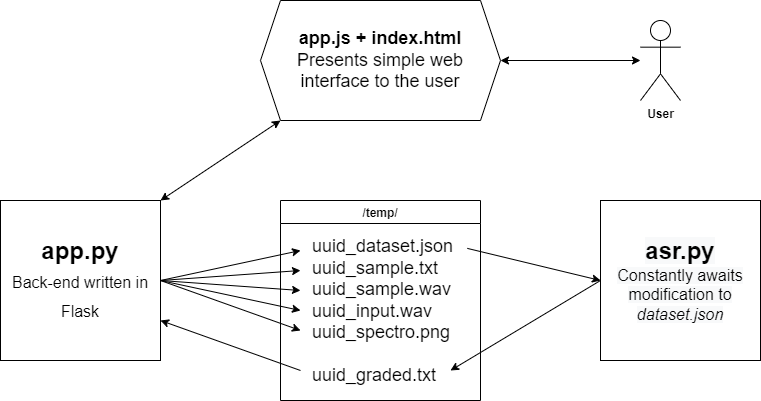
\includegraphics[scale=0.6]{images/workflow.png}

\newpage%######################################################################
\section*{Development Timeline}
\begin{itemize}
\item{Learn about ASR models and neural networks.}
\item{Learn about NeMo specifically.}
\item{Test ASR functions on Google Colab notebook.}
\item{Implement XML searching.}
\item{Assemble phrase libraries.}
\item{Shift from Colab notebook to local python app.}
\item{Design webpage using HTML.}
\item{Implement audio recording and save-to-file.}
\item{Implement Spectrogram creation w/ Librosa.}
\item{Get application to be fully functional locally}
\item{Shift application to UK AIC server.}
\item{Include ASR in program, check it has GPU access.}
\item{Sort out permissions so that all functions work from server.}
\item{Add Unique Universally Unique Identifiers (UUIDs) to all temporary files.}
\item{Test full functionality.}
\end{itemize}

\section*{Future Work}
\begin{itemize}
\item{Add a TTS tool that allows the user to hear how TTS would pronounce the prompt. This would be useful if the user encounters words with which they are not familiar. This could possibly be done with \textbf{pyttsx3} or \textbf{gTTS API}.}

\item{Add phrases in different languages, and the necessary support from the ASR. A small menu could let users switch the UI to other languages. Phrases can be added by simply enlarging the selection of \textit{dataset.xml} files.}

\item{Allow users to enter their own phrases with a text-entry box. This could be done with a basic HMTL \textit{Textbox}. Possible issues may arise from users entering non-standard characters, but this could just be prohibited to ensure at least the main functionality.}

\item{Allow the user to choose how their audio input is represented visually. For example, they could choose to see a wave plot instead of a spectrogram.}
\end{itemize}

\end{document}
